\documentclass[a4,a4paper]{article}
%\usepackage[active]{preview}
\input{~/mi-preamble-latex/mypreamble.tex}


\pagestyle{fancy}
\fancyhf{}
\chead{UTN Facultad Regional La Rioja - Esteban Bustamante}
\rhead{\includegraphics*[width=0.8cm]{/home/esbon1253/mi-preamble-latex/utnlogo.jpg}}
\cfoot{Propuesta - Trabajo Final}
\rfoot{\thepage}

\title{Propuesta - Trabajo Final }
\author{Esteban Bustamante - UTN Facultad Regional La Rioja}% \\ Profesor: Ing. Pedro Chahín Rearte}
\date{2024}


\begin{document}
\maketitle
\begin{center}
  \includegraphics[width=1\textwidth]{/home/esbon1253/mi-preamble-latex/utnlogo.jpg}
\end{center}

\pagebreak
\newpage

\tableofcontents

\pagebreak
\newpage

\section{Propuesta}
\label{sec:prop}

La idea en principio es hacer un sistema operativo de tiempo real enfocado a la realización del firmware de un bloque de hardware (a ser definido). En primer lugar se muestra en la figura \ref{fig:fig1} el sistema de microprocesadores con el que se va a trabajar. Estamos hablando de la placa PolarFire SoC FPGA Discovery Kit, que además de contener los procesadores mencionados, tiene una FPGA MPFS095T.


\begin{figure}[ht]
  \centering
  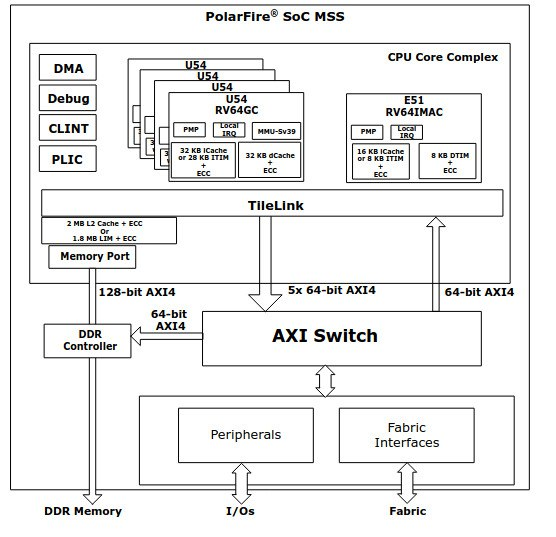
\includegraphics[width=1\textwidth]{figures/1.jpg}
  \caption{\label{fig:fig1} Subsistema de Microprocesadores}
\end{figure}

\par Como decía antes, la idea sería implementar en la FPGA algún bloque de hardware en la FPGA, idealmente ya verificado. Mi idea es sacar algún bloque de  \url{https://opencores.org/}, para de esa forma también dar a conocer comunidades open source. La duda en este momento es si el bloque estará más enfocado a DSP o a por ejemplo, procesamiento de imágenes o aceleradores de gráficos. Esto podría ser así haciendo uso de la materia Procesamiento Digital de Imágenes, puesto que me serviría como trabajo final de la misma el firmware de ese bloque.

\par El flujo sería el siguiente: primero lograría implementar el hardware en la FPGA, haciendo las adaptaciones necesarias, y luego las verificaciones formales de funcionamiento. En segundo lugar, definiría a grandes rasgos las tareas que llevaría adelante el firmware del bloque, para poder dimensionar correctamente el sistema operativo. Aquí comenzaría el proceso de diseño, seleccionando la mejor opción para el mismo. Teniendo en cuenta que el SoC es Linux capable, la idea es hacer un sistema bastante robusto, que por sobre todo sea inmune a la falla de servicios. La idea  sería hacer un microkernel, pensado como un RTOS, pero con la separación propia que implica un buen sistema operativo con microkernel, con la intención no solo de lograr una modularidad bastante grande, sino también de generar un sistema realmente escalable y donde sea posible diferenciar perfectamente el espacio de kernel del espacio de usuario, cosa que en muchos RTOS es un poco confuso. Por supuesto que viendo la arquitectura del sistema, corresponderá que el sistema operativo sea multi-core, corriendo sobre los 4 cores U64 tentativamente de forma asimétrica(AMP). Se hará uso de la plataforma provista por el fabricante de la placa, donde viene incluido entre otras cosas el bootloader. Finalmente, se hará el desarrollo del firmware del bloque propuesto además de por supuesto la capa de drivers y servicios que va a servir como middleware entre el kernel y la capa de aplicación, pero recordando siempre que estarán en modo usuario. Este sería el test inicial del S.O, y luego se hará un benchmark de distintos sistemas operativos compilados para la misma placa entre los cuales inicialmente se incluiría uno provisto por el fabricante, que es un Linux embebido generado con Yocto, y luego distintos RTOS de código abierto intentando configurarlos de una manera ``estándar'' 

\pagebreak
\newpage

\bibliographystyle{apacite}
\bibliography{bibliografia.bib}

\listoffigures

\end{document}
%%% Local Variables:
%%% mode: LaTeX
%%% TeX-master: t
%%% End:
